\documentclass[11pt]{article}
\usepackage[margin=0.75in]{geometry}
\usepackage[T1]{fontenc}
\usepackage{helvet}
\renewcommand{\familydefault}{\sfdefault}
\usepackage{tikz}
\usepackage{array}
\usepackage{enumitem}
\pagestyle{empty}
\setlength{\parindent}{0pt}
\raggedright  % even word spacing, easier to read
\hyphenpenalty=10000 \exhyphenpenalty=10000  % never split a word across lines
\setlist[enumerate,2]{label=(\alph*),leftmargin=2em,itemsep=1.8em}

% Build the key with:  pdflatex -jobname=<name>_KEY "\def\iskey{}\input{<name>}"
\newif\ifkey
\ifdefined\iskey \keytrue \fi
\newcommand{\ans}[1]{\ifkey\leavevmode{\color{red!75!black}#1}\fi}
\ifkey\setlist[enumerate,2]{label=(\alph*),leftmargin=2em,itemsep=0.6em}\fi

% ---------- helpers ----------
\newcommand{\tally}[1]{\tikz[baseline=0pt]{\foreach \i in {1,...,#1} \draw[line width=0.7pt] (\i*0.08,0) -- (\i*0.08,0.22);}}
% dot plot: \dotplot{min}{max}{value/count,...}{axis label}
\newcommand{\dotplot}[4]{%
\begin{tikzpicture}[x=0.9cm,y=0.33cm]
  \draw[thick] (#1-0.5,0) -- (#2+0.5,0);
  \foreach \t in {#1,...,#2} {\draw (\t,0.25) -- (\t,-0.25) node[below] {\t};}
  \foreach \v/\c in {#3} {\ifnum\c>0 \foreach \k in {1,...,\c} {\fill (\v,\k*1.15) circle (0.16cm);}\fi}
  \node at ({(#1+#2)/2},-2.3) {#4};
\end{tikzpicture}}

% blank number line, dots filled in on the key: \numline{min}{max}{label}{value/count,...}
\newcommand{\numline}[4]{%
\begin{tikzpicture}[x=0.9cm,y=0.33cm]
  \draw[thick] (#1-0.5,0) -- (#2+0.5,0);
  \foreach \t in {#1,...,#2} {\draw (\t,0.25) -- (\t,-0.25) node[below] {\t};}
  \node at ({(#1+#2)/2},-2.3) {#3};
  \path (#1,0) -- (#1,6);
  \ifkey\foreach \v/\c in {#4} {\ifnum\c>0 \foreach \k in {1,...,\c} {\fill[red!75!black] (\v,\k*1.15) circle (0.16cm);}\fi}\fi
\end{tikzpicture}}

\begin{document}

% The title is too long to share a line with Name, so Name goes above it
% (the same layout \lessontitle in handouts/preamble.tex uses for a long title).
\hfill Name \underline{\hspace{2in}}\par\vspace{0.5em}
{\Large\bfseries Frequency Tables, Dot Plots, and Histograms\ifkey\ \textcolor{red!75!black}{KEY}\fi}\par

\vspace{0.6em}
\textbf{Frequency} means how many times something happens. These three tools all show frequency.

\vspace{0.8em}
% ---------------- NOTES ----------------
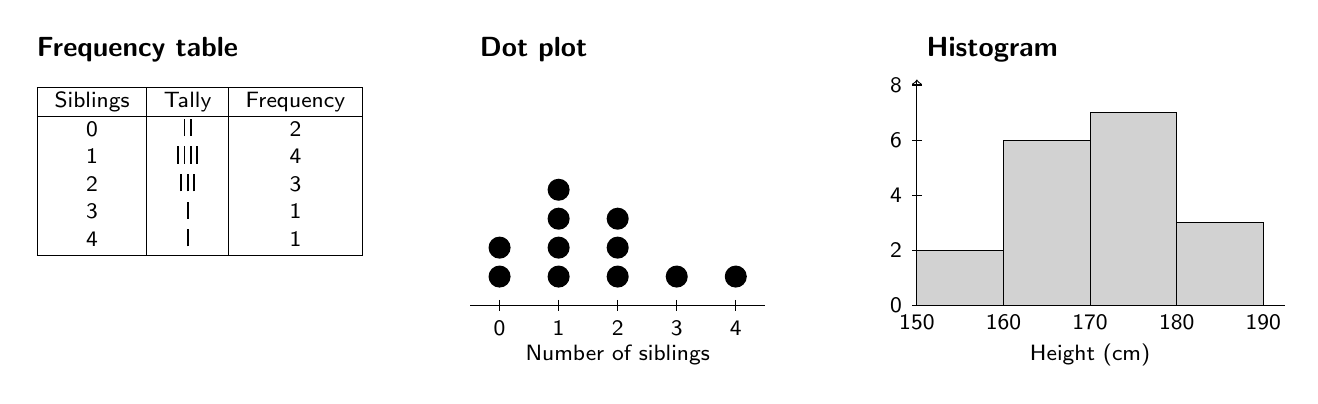
\begin{tikzpicture}
% frequency table example (same data as the dot plot)
\begin{scope}
  \node[anchor=west,font=\bfseries] at (0,3.25) {Frequency table};
  \node[anchor=north west,font=\footnotesize] at (0,2.9) {%
    \renewcommand{\arraystretch}{1.05}%
    \begin{tabular}{|c|c|c|}\hline
    Siblings & Tally & Frequency\\\hline
    0 & \tally{2} & 2\\ 1 & \tally{4} & 4\\ 2 & \tally{3} & 3\\ 3 & \tally{1} & 1\\ 4 & \tally{1} & 1\\\hline
    \end{tabular}};
\end{scope}
% dot plot example
\begin{scope}[xshift=6.0cm,x=0.75cm,y=0.35cm]
  \node[anchor=west,font=\bfseries] at (-0.5,9.3) {Dot plot};
  \draw (-0.5,0) -- (4.5,0);
  \foreach \t in {0,...,4} \draw (\t,0.2) -- (\t,-0.2) node[below,font=\footnotesize] {\t};
  \foreach \v/\c in {0/2,1/4,2/3,3/1,4/1} \foreach \k in {1,...,\c} \fill (\v,\k*1.05) circle (0.14cm);
  \node[font=\footnotesize] at (2,-1.8) {Number of siblings};
\end{scope}
% histogram example
\begin{scope}[xshift=11.3cm,x=0.55cm,y=0.35cm]
  \node[anchor=west,font=\bfseries] at (0,9.3) {Histogram};
  \draw[->] (0,0) -- (0,8.2); \draw (0,0) -- (8.5,0);
  \foreach \y in {0,2,...,8} \draw (0.12,\y) -- (-0.12,\y) node[left,font=\footnotesize] {\y};
  \foreach \i/\h in {0/2,1/6,2/7,3/3} \draw[fill=gray!35] (\i*2,0) rectangle (\i*2+2,\h);
  \foreach \i/\l in {0/150,1/160,2/170,3/180,4/190} \node[below,font=\footnotesize] at (\i*2,0) {\l};
  \node[font=\footnotesize] at (4,-1.8) {Height (cm)};
\end{scope}
\end{tikzpicture}

\vspace{0.4em}
\renewcommand{\arraystretch}{1.35}
\begin{tabular}{|>{\raggedright}p{2.1in}|>{\raggedright}p{2.1in}|>{\raggedright\arraybackslash}p{2.1in}|}
\hline
Each \textbf{value} gets a row. &
Each \textbf{value} gets a spot on a number line. &
Values are put in \textbf{groups} (bins). \\
Make a tally mark for each data point, then count. &
\textbf{One dot = one data point.} Stack the dots. &
Bars \textbf{touch}. No gaps between groups. \\
Frequency column = how many. &
Height of the stack = how many. &
Bar height = how many in that group. \\
\hline
\end{tabular}

\vspace{0.8em}
\textbf{Histogram rule:} If a number is \textbf{on a line} between two bars, it goes in the bar on the \textbf{right}.
Example: 160 goes in the 160 to 170 bar.

\vspace{0.4em}
The frequency table and dot plot above show the \textbf{same data}. Check: 2 + 4 + 3 + 1 + 1 = 11 students.

\vspace{0.4em}
\textbf{Every time you read a graph:} read the title, read both axis labels, then check the scale.

\vspace{0.4em}
Work with a partner. Compare answers when you finish each problem.

% ---------------- PROBLEMS ----------------
\vspace{1.0em}
\begin{enumerate}[leftmargin=1.5em,itemsep=1em]

\item This dot plot shows how many pets some students have.

\begin{center}\dotplot{0}{5}{0/4,1/6,2/3,3/2,4/0,5/1}{Number of pets}\end{center}
\begin{enumerate}
  \item How many students have exactly 2 pets? \ans{\quad 3}
  \item How many students are in the data? \ans{\quad 4 + 6 + 3 + 2 + 0 + 1 = 16}
  \item How many students have more than 2 pets? \ans{\quad 2 + 0 + 1 = 3}
  \item What number of pets is most common? \ans{\quad 1 pet}
\end{enumerate}
\vspace{1.5em}

\newpage
\item A soccer team scored these goals in 12 games. Make a dot plot.

\begin{center}
2,\; 0,\; 1,\; 3,\; 1,\; 1,\; 4,\; 2,\; 0,\; 1,\; 2,\; 1

\vspace{0.5em}
\numline{0}{5}{Goals scored in a game}{0/2,1/5,2/3,3/1,4/1}
\end{center}

\item 20 students said how many siblings they have. Make a frequency table.

\begin{center}
1,\; 2,\; 0,\; 3,\; 1,\; 1,\; 2,\; 4,\; 0,\; 2,\; 1,\; 3,\; 2,\; 1,\; 0,\; 2,\; 1,\; 5,\; 2,\; 1

\vspace{0.6em}
\renewcommand{\arraystretch}{1.3}
\begin{tabular}{|c|p{1.4in}|p{0.9in}|} \hline
Siblings & Tally & Frequency \\ \hline
0 & \ans{\tally{3}} & \ans{3} \\ 1 & \ans{\tally{7}} & \ans{7} \\ 2 & \ans{\tally{6}} & \ans{6} \\ 3 & \ans{\tally{2}} & \ans{2} \\ 4 & \ans{\tally{1}} & \ans{1} \\ 5 & \ans{\tally{1}} & \ans{1} \\ \hline
\end{tabular}
\end{center}
\begin{enumerate}[itemsep=\ifkey 0.6em\else 1.4em\fi]
  \item How many students have 2 or more siblings? \ans{\quad 6 + 2 + 1 + 1 = 10}
  \item How can you use your table to check that you counted everyone? \ans{\quad Add the frequencies. Total = 20.}
\end{enumerate}
\vspace{0.4em}

\item This frequency table shows how many hours some students slept last night.

\vspace{0.3em}
\begin{minipage}[t]{0.33\linewidth}\vspace{0pt}\centering
\begin{tabular}{|c|c|} \hline
Hours of sleep & Frequency \\ \hline
5 & 2 \\ 6 & 4 \\ 7 & 6 \\ 8 & 5 \\ 9 & 3 \\ \hline
\end{tabular}
\end{minipage}\hfill
\begin{minipage}[t]{0.62\linewidth}\vspace{0pt}
\begin{enumerate}[itemsep=\ifkey 1em\else 2.2em\fi]
  \item How many students are in the data? \ans{\quad 20}
  \item How many students slept less than 7 hours? \ans{\quad 2 + 4 = 6}
\end{enumerate}
\end{minipage}

\vspace{1.2em}
\begin{enumerate}[start=3]
  \item Make a dot plot of the same data.

  \begin{center}\numline{4}{10}{Hours of sleep}{5/2,6/4,7/6,8/5,9/3}\end{center}
\end{enumerate}

\newpage
\item This histogram shows how many minutes some students take to get to school.

\begin{center}
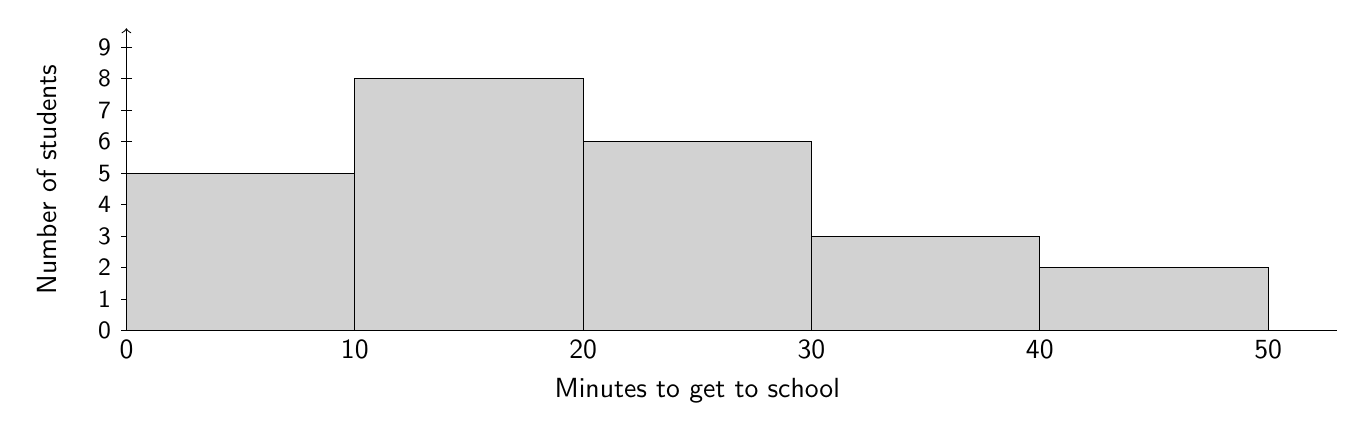
\begin{tikzpicture}[x=0.29cm,y=0.4cm]
  \draw[->] (0,0) -- (0,9.6); \draw (0,0) -- (53,0);
  \foreach \y in {0,...,9} \draw (0.25,\y) -- (-0.25,\y) node[left,font=\small] {\y};
  \foreach \i/\h in {0/5,1/8,2/6,3/3,4/2} \draw[fill=gray!35] (\i*10,0) rectangle (\i*10+10,\h);
  \foreach \l in {0,10,...,50} \node[below] at (\l,0) {\l};
  \node[rotate=90] at (-3.5,4.8) {Number of students};
  \node at (25,-1.9) {Minutes to get to school};
\end{tikzpicture}
\end{center}
\begin{enumerate}
  \item How many students take from 20 to 30 minutes? \ans{\quad 6}
  \item How many students take less than 20 minutes? \ans{\quad 5 + 8 = 13}
  \item How many students are in the data? \ans{\quad 5 + 8 + 6 + 3 + 2 = 24}
  \item Can you tell from this graph how many students take exactly 15 minutes? Explain.

  \ans{No. The graph only shows that 8 students take from 10 to 20 minutes. It hides the exact values.}
\end{enumerate}
\vspace{1.5em}

\item A basketball player scored these points in 15 games.

\begin{center}
12,\; 8,\; 15,\; 21,\; 9,\; 14,\; 18,\; 10,\; 25,\; 13,\; 7,\; 16,\; 20,\; 11,\; 19
\end{center}
\begin{enumerate}[itemsep=1em]
  \item Make a frequency table. Count how many games are in each group. Remember the histogram rule.

  \begin{center}
  \renewcommand{\arraystretch}{1.6}
  \begin{tabular}{|c|p{2in}|} \hline
  Points & Frequency \\ \hline
  5 to 10 & \ans{3 \;(7, 8, 9)} \\ 10 to 15 & \ans{5 \;(10, 11, 12, 13, 14)} \\ 15 to 20 & \ans{4 \;(15, 16, 18, 19)} \\ 20 to 25 & \ans{2 \;(20, 21)} \\ 25 to 30 & \ans{1 \;(25)} \\ \hline
  \end{tabular}
  \end{center}
  \item Make a histogram. Label both axes.

  \begin{center}
  \begin{tikzpicture}[x=0.38cm,y=0.42cm]
    \draw[->] (0,0) -- (0,6.6); \draw (0,0) -- (30,0);
    \foreach \y in {0,...,6} \draw (0.2,\y) -- (-0.2,\y) node[left,font=\small] {\y};
    \foreach \l/\p in {5/3,10/8,15/13,20/18,25/23,30/28} {\draw (\p,0.2) -- (\p,-0.2) node[below] {\l};}
    \ifkey\begin{scope}[red!75!black]
      \foreach \i/\h in {0/3,1/5,2/4,3/2,4/1} \draw[fill=red!12] (3+\i*5,0) rectangle (8+\i*5,\h);
      \node[rotate=90] at (-2.6,3) {Games};
      \node at (15.5,-1.9) {Points scored};
    \end{scope}\fi
  \end{tikzpicture}
  \end{center}
\end{enumerate}

\end{enumerate}

\end{document}
